\documentclass{llncs}
\usepackage{graphicx}

%
\begin{document}

\title{Mass surveillance in cyberspace and the lost art of keeping a secret}
\subtitle{Policy lessons for nation-states after the Snowden leaks}

\author{Theo Tryfonas\inst{1} \and Michael Carter\inst{2} \and Tom Crick\inst{3} \and Panagiotis Andriotis\inst{1}}
\institute{Crypto Group, University of Bristol, UK\\
\email {t.tryfonas@bristol.ac.uk, p.andriotis@bristol.ac.uk}
\and
Surveillance Studies Centre, Queen's University, Canada\\
\email{michael.carter@queensu.ca} 
\and
Dept. of Computing, Cardiff Metropolitan University, UK\\
\email{tcrick@cardiffmet.ac.uk}}

\maketitle

\begin{abstract}
Global security concerns, acts of terrorism and organised crime activity have motivated nation states to delve into implementing measures of mass surveillance in cyberspace, the breadth of which was partly revealed by the whistleblower Edward Snowden. But are modern nation states fighting a battle in the wrong space? Is mass surveillance of cyberspace effective and are the conventional metaphors of technology control appropriate for it? Can algorithms detect, classify and decide effectively on what constitutes suspicious activity? We argue that as cyberspace is a construct that has only recently been viewed strategically, let alone indoctrinated (the UK’s cyber-security strategy is only 4 years old), the societal impact of such bulk measures is yet much unclear – as are the assumptions about the fitness of state organisations that are charged with their oversight and the potential for unintended consequences. Recent experiences highlight the role of multiple forms of intelligence inputs, especially human- and community-based, and the need for application of such intrusive measures in a targeted manner. We believe that intrusive measures, where necessary, must be used decoupled from the seductive promises of advanced technology and ought to go hand-in-hand with means that strengthen the affected communities to identify, report and battle extremism and organised crime, in ways that safeguard the fundamental principles of our contemporary democratic Western states.
\keywords{Surveillance, cyberspace, public trust}
\end{abstract}

\section{Introduction}
\label{sec:Introduction}
In the fall of 2014, UN Special Rapporteur Ben Emmerson submitted his report on practices of mass surveillance by state actors and the threat that this approach to intelligence gathering poses to universal civil and political rights \cite{Emerson}. Emmerson called for open and transparent discussion between government and citizens to inform and determine an appropriate balance between public security and personal privacy. The Special Rapporteur pointed out that what is technologically possible is not necessarily desirable or responsible. This is an argument that surveillance scholars such as Kirstie Ball have been making for several years now \cite{Ball}. However, traction for this debate was limited until June 2013 when files leaked by NSA whistleblower Edward Snowden were published in the Guardian by journalist Glenn Greenwald. 

Two years after the initial release of Snowden files, surveillance legislation remains highly contested in Canada, the US and the UK. Perhaps most notably is the sunsetting of section 215 of The Patriot Act and subsequent passing of The Freedom Act in the United States in early June \cite{Patriot}. Days later the Senate of Canada passed controversial anti-terrorism Bill C-51, which received sustained public opposition from big business, journalists, law professors, activists and the privacy commissioner \cite{C-51}. A week prior to these developments the latest rendition of ’the snooper’s charter’ in the UK was announced in the Queen’s speech. Former deputy Prime Minister Nick Clegg publicly opposed the legislation, currently known as The Investigatory Powers Bill, arguing it threatens the privacy rights of citizens.  

These measures are indicative state attempts to curb terrorism threats by enabling the development of surveillance capabilities that are of bulk collection nature, rather than targeted to specific individuals. Proponents of these argue that the proliferation of high technology, including anonymity, cryptography and secure communication tools, enables organised crime to communicate safely and go undetected. On the other hand privacy activists advocate the fundamental need for safe spaces to develop one's ideas, the human right to privacy and an individual's need to protect themselves from abusive regimes.

In this paper we develop an argument about the place of mass cyberspace surveillance in society. We believe that deployment of intrusive systems on line, where necessary, should be of clear and transparent purpose to the public and accompanied by measures that empower the affected communities to tackle the root causes of concern, e.g. radicalisation, hate speech etc. Drawing on analogies from other surveillance systems we develop the idea of co-creation of surveillance, in the civic innovation sense of the term, arguing that otherwise Western states risk developing non-transparent and unaccountable structures of power that undermine the fundamental values of their civilisation.

The rest of the paper is organised as follows: section \ref{sec:Background} provides some further background to the issue of mass surveillance of cyberspace in the West and discusses aspects of the Snowden leaks; section \ref{sec:Understanding} develops some fundamental ideas and draws on analogies from other domains to explore the difficulties and challenges; section \ref{sec:Creating} introduces our ideas for a system-of-systems approach and co-creation of intrusive technologies and finally we conclude with section \ref{sec:Conclusions}.

\section{Background}
\label{sec:Background}
The debate on mass surveillance, which is comprised of several threads, has engaged a range of social groups including politicians, law makers, journalists, academics, tech firms, activists, artists and the general public. The term mass surveillance is used to distinguish the bulk collection of data from targeted surveillance, which typically involves a 'person of interest'. Central to this aspect of the debate is the legal warrant, which is traditionally issued upon satisfaction of a certain level of suspicion. In the case of Canada, for example, Bill C-13, which was passed in the fall of 2014, significantly lowered the level of suspicion required to justify the collection of personal data. Bill C-13 also addressed the distinction between data and meta data, which is a hotly debated topic in surveillance legislation. Advocates of expanded surveillance powers for the state have attempted to mollify concerns by arguing that meta data does not threaten the political or civil rights of citizens because it is data about communication and not the content of communication. This argument has been routinely problematized by opponents who point out that metadata can reveal religious beliefs, political leanings and intimate relationships. Moreover, meta data is used by state actors to kill people, as was famously announced by former NSA and CIA director Michael Hayden \cite{Hayden}. 

As legislation governing surveillance practices in Western society continues to evolve, a related debate is emerging. In early June, UN Special Rapporteur David Kaye submitted his report on the right to freedom of opinion and expression. Kaye argued that encryption and anonymity in digital communications is fundamental for the preservation of privacy and the protection of opinion and belief. The Special Rapporteur framed encrypted communication as a tool for citizens to protect their human rights from infringement by government agencies. Moreover, he called for the mobilization of state resources to ensure all individuals using digital communication can do so with encryption. Just prior to the release of the report, Nico Sell, co-founder of leading encryption app Wickr, launched a non-profit organization with this goal in mind. 

However, less popular apps like Wickr and more mainstream services like WhatsApp and Snapchat are being targeted by government. In January 2015 British Prime Minister David Cameron publicly announced his intention to ban communications that are not accessible by government agencies. Cameron asked for and quickly received support for this position from President Obama. The movement to ban encryption points towards the criminalization of private communication, which would threaten a variety of political, civil and human rights. Moreover, security experts have noted that weakening communication by demanding back door access will increase vulnerabilities and by extension could compromise national security. In May 2015 over 140 tech firms including Apple, Google and Symantec sent an open letter to Obama urging him not to push for government access to encrypted communication. In the meantime, apps that offer individuals encrypted communication are proliferating as concern for privacy in mainstream society climbs.

The Snowden leaks revealed a wide portfolio of projects and initiatives both from the NSA in the US and GCHQ in the UK. These range from specific data collection projects such as Optic Nerve, aimed at Yahoo! webcam traffic, to influencing the development of cryptographic standards to contain vulnerabilities, so they can be penetrated easier \cite{ECDH}. In this varied context the Anderson report \cite{Anderson} that was released recently as a comprehensive review of the UK's capabilities and practice prior to revamping the existing legislation, emphasised a number of issues, amongst the most important - and contested - of which, was the suggestion for judicial rather than ministerial oversight.

Politicians have already started countering the suggestion by claiming that despite the wide and varied nature of operations, ministers can have more topical information than judges and make decisions quicker, as opposed to going through the overheads of a judiciary procedure. However, due to the wide reach of operations and their varied nature it is questionable how much in depth understanding can law makers develop in the short amounts of time to decide in the absence of a transparent and well defined process. Another interesting point raised after the leaks is about the level of access and trust vested to a third-party, private contractor by security services, which may be indicative of the lack of resourcing of the relevant agencies -- and adding to the need for sufficient oversight.
%(\ref{fig:Yahoo})
\begin{figure}
\begin{center}
\label{fig:Yahoo}
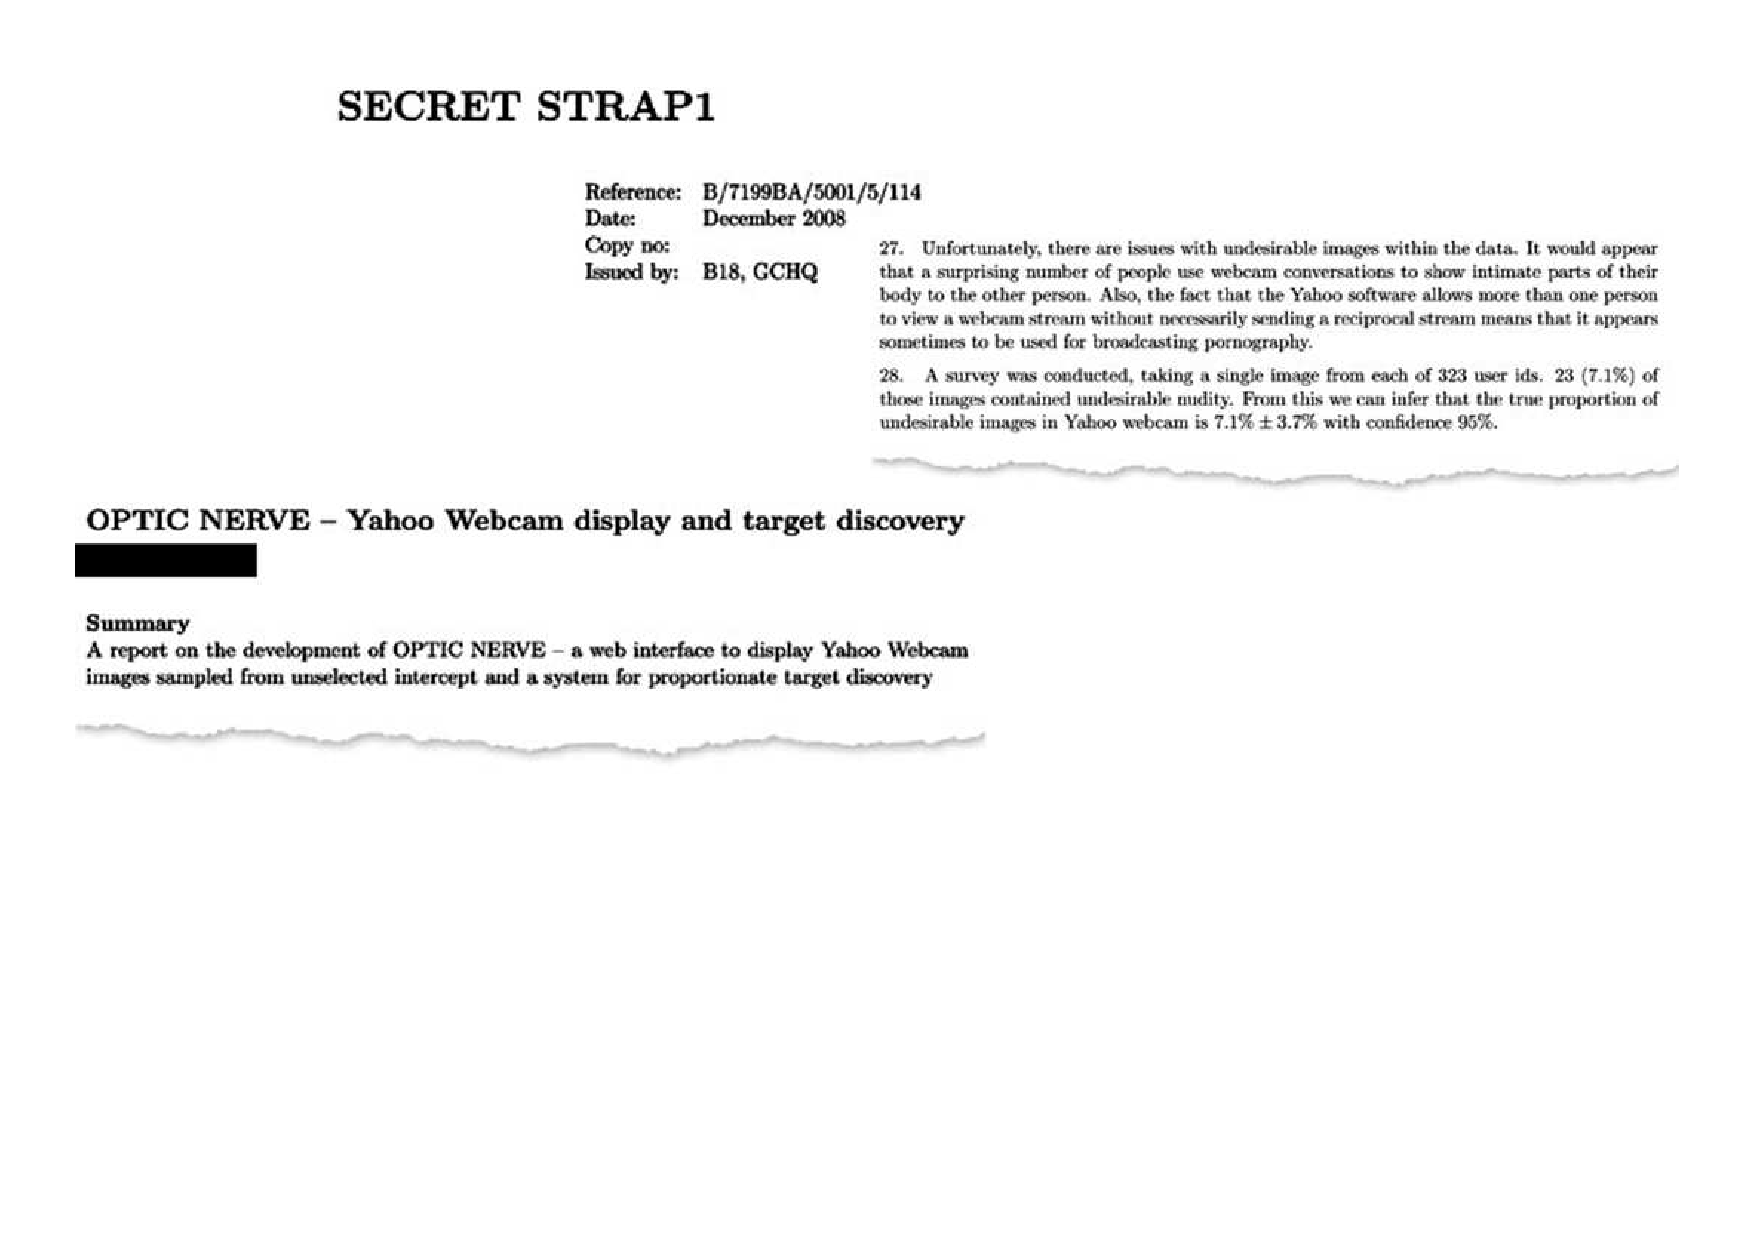
\includegraphics[scale=0.3]{fig1}
\caption{Yahoo! webcam traffic monitoring report snapshots from Snowden's cache.}
\end{center}
\end{figure}

\section{Public understanding of surveillance and the context of cyberspace}
\label{sec:Understanding}
\subsection{Deconstructing State imagery of surveillance}
Politicians use many metaphors and analogies to promote the idea of cyberspace surveillance among the public. David Cameron, the UK Prime Minister, talked in early 2015 about the need for the state to be able to eavesdrop digital communications over the Internet, just as it can happen over the telephony network. Drawing on analogies between the more familiar phone technology and the public's understanding of a legitimate wire-tapping process, he tried to reach out to the public, constructing an image of accepted mass surveillance. Among political circles one of the most used analogies for constructing relevant images is the case of the closed-circuit television (CCTV) surveillance systems. This is a familiar, and very tangible, system which in the UK at least enjoys large amounts of public tolerance and even approval \ref{}. XXXXXXXXXX more numbers etc. here XXXXXXXXXXXXXX

xx

Metaphors and analogies for public understanding of surveillance in cyberspace. The analogy of CCTV. Wide sensing surface and algorithmic determination. Challenges from unintended consequences of bulk data collection. Algorithmic determination failures. Asumptions of strong governance.
\subsection{The personal data dimension}
Monetisation/commoditisation of personal data resulting in casualisation of privacy rights. Unclear operating frameworks and private sector abuse of data. How it contributes to indifference and acceptance of surveillance - but could provide an opportunity for better surveillance!

\section{Co-creating viable surveillance systems}
\label{sec:Creating}
Confusion of purpose by inappropriate use of metaphors. Need to intervene earlier in the radicalisation lifecycle to debunk the propaganda messages and appeal of radicalism. Need for human-centric intelligence, open source and targeted operations.

The example of CCTV in the UK as a system-of-systems. The need for education and public understanding of surveillance tech. Implications for co-creation with the community.

\section{Conclusions}
\label{sec:Conclusions}
In light of global security challenges that include radicalisation and terrorism, but also increasing use of high technology by organised transnational crime, it is tempting for national states and their security services to develop mass surveillance programmes. The seductive promise of technological capability however, may not be a solution that is as relevant as human centric intelligence, as both wide surface scanning and artificial intelligence face their challenges as we've argued. And in any case this kind of capability is retrospective and missing the crucial stage of early intervention at the root cause of phenomena such as radicalisation of young persons to jihadist ideologies.

Creating powerful capabilities with insufficient oversight increases the potential for abuse of power and risks the loss of confidence and support from the wider public. This is exactly one of the aims of dissident groups and so we believe that organised states should refrain from developing surveillance capabilities in absentia of their key stakeholders, particularly the wider public. It is only with public trust that these may be successfully deployed. It is also essential that the paradigm of their development is one of a system-of-systems, i.e. viewed as an integral part of the wider state capability for countering terrorism and other organised crime. The whole picture ought to include early intervention to counter and debunk the appealing propaganda of terror groups and also to enable affected communities to report to and cooperate with the relevant authorities in confidence.

It is tempting for security services to explore every avenue of technology to counter such a severe threat. But the resulting programmes ought to respect fundamental rights of Western democracies, operate under strict due diligence and be accepted by the public, much like the example of CCTV in Britain. For, if the state in the process creates inadvertently the Matrix, it ought to be aware that the next historic revolution may come exactly from within it.

%
% ---- Bibliography ----
%
\begin{thebibliography}{}
%
\bibitem{Emerson} %2clar:eke}
Emerson, B.:
Annual report of the Special Rapporteur to the Human Rights Council, March 2014

\bibitem{Ball}
Ball, C.:
Organization, surveillance and the body: Towards a politics of resistance. In: Lyon, David ed. Theorising Surveillance: The Panopticon and beyond. Collumpton, UK: Willan Publishing. 

\bibitem{Patriot}
Kelly, E.:
Senate approves USA Freedom Act, Usa Today,  June 2, 2015

\bibitem{C-51}
House of Commons of Canada:
Bill C-51, first reading, January 30, 2015

\bibitem{Hayden}
Ferran, L.:
Ex-NSA Chief: 'We Kill People Based on Metadata', abcNEWS, May 12, 2014

\bibitem{ECDH}
Hales, T.:
The NSA Back Door to NIST, Notices of the AMS, Vol. 61, No 2, 191--192

\bibitem{Anderson}
Anderson, D.:
A Question of Trust -– Report of the Investigatory Powers Review, Independent Reviewer of Terrorism Legislation, June 11, 2015

\end{thebibliography}
\end{document}